\documentclass[12pt,preprint]{aastex}

% has to be before amssymb it seems
\usepackage{color,hyperref}
\definecolor{linkcolor}{rgb}{0,0,0.5}
\hypersetup{colorlinks=true,linkcolor=linkcolor,citecolor=linkcolor,
            filecolor=linkcolor,urlcolor=linkcolor}

\usepackage{url}
\usepackage{algorithmic,algorithm}
\usepackage{multirow}

\usepackage{listings}
\definecolor{lbcolor}{rgb}{0.9,0.9,0.9}
\lstset{language=Python,
        basicstyle=\footnotesize\ttfamily,
        showspaces=false,
        showstringspaces=false,
        tabsize=2,
        breaklines=false,
        breakatwhitespace=true,
        identifierstyle=\ttfamily,
        keywordstyle=\bfseries\color[rgb]{0.133,0.545,0.133},
        commentstyle=\color[rgb]{0.133,0.545,0.133},
        stringstyle=\color[rgb]{0.627,0.126,0.941},
    }

\usepackage{amssymb,amsmath}

\newcommand{\project}[1]{{\sffamily #1}}
\newcommand{\Python}{\project{Python}}
\newcommand{\numpy}{\project{numpy}}
\newcommand{\bart}{\project{Bart}}
\newcommand{\emcee}{\project{emcee}}
\newcommand{\kepler}{\project{Kepler}}
\newcommand{\license}{MIT License}

\newcommand{\paper}{\emph{Article}}

\newcommand{\foreign}[1]{\emph{#1}}
\newcommand{\etal}{\foreign{et\,al.}}
\newcommand{\etc}{\foreign{etc.}}

\newcommand{\Fig}[1]{Figure~\ref{fig:#1}}
\newcommand{\fig}[1]{\Fig{#1}}
\newcommand{\figlabel}[1]{\label{fig:#1}}
\newcommand{\Tab}[1]{Table~\ref{tab:#1}}
\newcommand{\tab}[1]{\Tab{#1}}
\newcommand{\tablabel}[1]{\label{tab:#1}}
\newcommand{\Eq}[1]{Equation~(\ref{eq:#1})}
\newcommand{\eq}[1]{\Eq{#1}}
\newcommand{\eqlabel}[1]{\label{eq:#1}}
\newcommand{\Sect}[1]{Section~\ref{sect:#1}}
\newcommand{\sect}[1]{\Sect{#1}}
\newcommand{\App}[1]{Appendix~\ref{sect:#1}}
\newcommand{\app}[1]{\App{#1}}
\newcommand{\sectlabel}[1]{\label{sect:#1}}
\newcommand{\Algo}[1]{Algorithm~\ref{algo:#1}}
\newcommand{\algo}[1]{\Algo{#1}}
\newcommand{\algolabel}[1]{\label{algo:#1}}

% math symbols
\newcommand{\dd}{\ensuremath{\,\mathrm{d}}}
\newcommand{\bvec}[1]{\ensuremath{\boldsymbol{#1}}}
\newcommand{\unit}[1]{\ensuremath{\mathrm{#1}}}
\newcommand{\normal}[1]{\ensuremath{\mathcal{N}(#1)}}

\newcommand{\obs}[1]{\ensuremath{\overline{#1}}}

% abstract parameters
\newcommand{\hyperhyper}{\ensuremath{\lambda}}
\newcommand{\hyper}{\ensuremath{\theta}}
\newcommand{\local}{\ensuremath{w}}
\newcommand{\data}{\ensuremath{x}}

% hierarchical parameters
\newcommand{\rpop}{\ensuremath{\alpha}}
\newcommand{\Rpop}{\ensuremath{\beta}}
\newcommand{\selection}{\ensuremath{\delta}}

% PGM parameters
\newcommand{\rp}{\ensuremath{r}}
\newcommand{\ror}{\ensuremath{z}}
\newcommand{\rorobs}{\obs{\ror}}
\newcommand{\Rs}{\ensuremath{R}}
\newcommand{\Rsobs}{\obs{\Rs}}
\newcommand{\sigmasobs}{\obs{\sigma}}
\newcommand{\sn}{\ensuremath{\Sigma}}
\newcommand{\isobs}{\obs{q}}

% Selection parameters
\newcommand{\Pmax}{\ensuremath{P_\mathrm{max}}}
\newcommand{\selectwidth}{\ensuremath{\Delta}}
\newcommand{\snmin}{\ensuremath{\Sigma_\mathrm{min}}}


\begin{document}

\title{%
    Probabilistic hierarchical modeling of exoplanet populations using
    incomplete catalogs
}

\newcommand{\nyu}{2}
\newcommand{\mpia}{3}
\author{%
    Daniel~Foreman-Mackey\altaffilmark{1,\nyu},
    David~W.~Hogg\altaffilmark{\nyu,\mpia},
    \etal
}
\altaffiltext{1}{To whom correspondence should be addressed:
                        \url{danfm@nyu.edu}}
\altaffiltext{\nyu}{Center for Cosmology and Particle Physics,
                        Department of Physics, New York University,
                        4 Washington Place, New York, NY, 10003, USA}
\altaffiltext{\mpia}{Max-Planck-Institut f\"ur Astronomie,
                        K\"onigstuhl 17, D-69117 Heidelberg, Germany}

\begin{abstract}



\end{abstract}

\keywords{%
}

\section{Introduction}


\section{A toy model}

We start by assuming that ever target star has some $K$ orbiting planets.
Most of these planets are unobserved because they are two small to be
detectable or because of geometry.
The graphical model in \fig{gm} is a sketch of the hypothetical generative
procedure for a catalog of exoplanet observations.
The way it is shown, this model is extremely general but we will consider a
very specific form here.
In \fig{gm} the global ``hyper'' parameters are:
\begin{itemize}
\item{the parameters describing the distributions of the exoplanet population
\population, and}
\item{the parameters of a model of the catalog's exoplanet selection function
\selection.}
\end{itemize}
Similarly, the ``hidden variables'' are:
\begin{itemize}
\item{the physical parameters of the star and the stellar system
\stellar---including the stellar mass and radius, a measure of the stellar
variability, and the mean inclination of the orbiting exoplanets---and}
\item{the physical parameters of an exoplanet \planet---period, radius, and
relative inclination.}
\end{itemize}
Finally, the observables are

\begin{figure}[htbp]
\begin{center}
    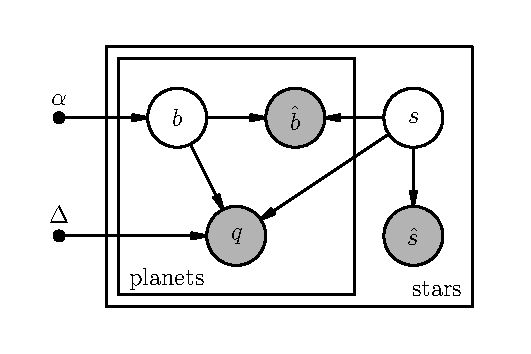
\includegraphics{gm.pdf}
\end{center}
\caption{%
\figlabel{gm}}
\end{figure}

\begin{deluxetable}{ccl}
\tablecaption{%
A description of the model parameters.
\tablabel{parameters}}
\tablewidth{0pt}
\tablehead{& & \colhead{Description}}
\startdata
\multirow{3}{*}{\population}
& $\population_\period$ & The period distribution \\
& $\population_\radius$ & The exoplanet radius distribution \\
& $\population_\relincl$ & The relative inclination distribution \\
\hline
\selection & --- & The parameters of the catalog selection function \\
\hline
$\isobs_{kn}$ & --- & A flag indicating the presence of exoplanet $k$ orbiting
star $n$ in the catalog \\
\hline
\multirow{3}{*}{$\planet_{kn}$}
& $\period_{kn}$ & The period of exoplanet $k$ orbiting star $n$ (or null) \\
& $\radius_{kn}$ & The exoplanet's radius \\
& $\relincl_{kn}$ & The inclination of this orbit away from the systemic mean \\
\hline
\multirow{3}{*}{$\planetobs_{kn}$}
& $\periodobs_{kn}$ & The observed exoplanet period and uncertainty \\
& $(\rorobs)_{kn}$ & The observed radius ratio and uncertainty \\
& $\impactobs_{kn}$ & A constraint on the observed impact parameter \\
\hline
\multirow{4}{*}{$\stellar_{n}$}
& $\smass_{n}$ & The mass of star $n$ \\
& $\sradius_{n}$ & The radius of star $n$ \\
& $\snoise_{n}$ & The ``variability'' of star $n$ \\
& $\incl_{n}$ & The mean inclination of the exoplanets in the system $n$ \\
\hline
\multirow{2}{*}{$\stellarobs_{n}$}
& $\sloggobs_{n}$ & The observed surface gravity (and uncertainty) of star $n$ \\
& $\snoiseobs_{n}$ & The estimated variability of star $n$ \\
\enddata
\end{deluxetable}

\acknowledgments
SAMSI. %
It is a pleasure to thank
    \ldots
for helpful contributions to the ideas and code presented here.
This project was partially supported by the NSF (grant AST-0908357), and NASA
(grant NNX08AJ48G).

\newcommand{\arxiv}[1]{\href{http://arxiv.org/abs/#1}{arXiv:#1}}
\begin{thebibliography}{}\raggedright

\bibitem[Fang \& Margot(2012)]{fang}
Fang, J., \& Margot, J.-L.\ 2012, \apj, 761, 92
\arxiv{1207.5250}

\bibitem[Tremaine \& Dong(2012)]{tremaine}
Tremaine, S., \& Dong, S.\ 2012, \aj, 143, 94
\arxiv{1106.5403}

\end{thebibliography}

\end{document}
